\chapter{Metodologia}
\label{sec:metodologia}

Neste capítulo será apresentada a metodologia de pesquisa adotada para desenvolvimento 
deste trabalho de conclusão de curso bem como o problema a ser resolvido, a hipótese 
levantada a partir do problema, seus objetivos e justificativa.

\section{Pesquisa-ação}

A pesquisa-ação ou action-research surgiu na década de 1940, no contexto de críticas ao uso
de procedimentos clássicos de ciências naturais na pesquisa social por razões de ordem prática 
(conhecimento teórico gerado teria pouca aplicabilidade na prática) ou ideológica (pesquisas estariam
sendo realizadas como uma forma de controle social)\cite{gil2010metodos}.

O pesquisador na pesquisa-ação
assume como premissa que processos sociais complexos, como a interação
entre organizações e seus sistemas de informação, são melhor investigados
quando se introduzem mudanças nestes processos e se observa os efeitos
destas mudanças. Outra premissa é que estes processos devem ser
investigados como uma entidade completa, não sendo possível extrair o objeto
de investigação do seu contexto. Desta forma, na pesquisa-ação busca-se avançar na teoria 
atuando na prática, o que é feito através de
ações no contexto de uma organização específica. O foco do pesquisador é na
compreensão do problema e das ações realizadas para solucioná-lo dentro de
um ambiente real particular e não na verificação de uma hipótese de caráter
geral num ambiente de laboratório~\cite{fuks2008suporte}.

\begin{figure}[htpb]
 \begin{center}
    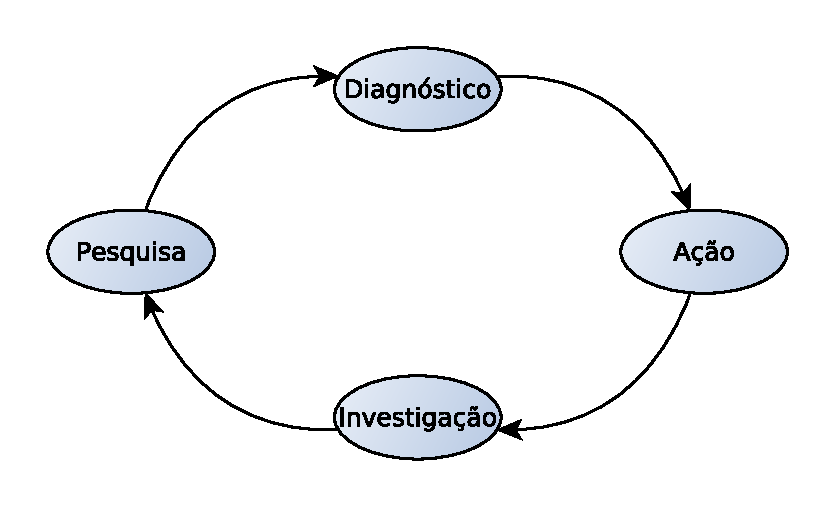
\includegraphics[width=.70\textwidth]{figuras/pesquisa-acao.eps}
 \end{center}
  \caption{Ciclo de desenvolvimento da pesquisa-ação}
  \label{fig:pesquisa-acao}
\end{figure}

Segundo Ana Paula~\cite{dos2012aplicaccao} "O pesquisador pode ter uma visão de \emph{insider}
ou \emph{outsider}, na realização de uma pesquisa-ação.
A visão de um \emph{insider} ocorre quando o pesquisador vivencia o problema e o traz para a pesquisa,
ou seja leva seus problemas para realizar a pesquisa, já a visão de outsider é quando a instituição
tem um problema e chama um pesquisador ou o pesquisador vai atrás de uma empresa ou cenário
real que tenha o problema". 

No caso desta pesquisa, estarei dentro de um contexto de 
desenvolvimento para o governo por participar do Projeto do Novo Portal do Software
Público, desta forma a pesquisa pode ser classificada como \emph{insider}.


\subsection{Abordagem Quantitativa versus Qualitativa}

As pesquisas, conforme as abordagens metodológicas que englobam, são classificadas em
dois grupos distintos – o quantitativo e o qualitativo. O primeiro obedece ao paradigma
clássico (positivismo) enquanto o outro segue o paradigma chamado alternativo~\cite{terence2006abordagem}.

\begin{table}[htb]
\center
\footnotesize
\begin{tabular}{|p{4cm}|p{5cm}|p{5cm}|}
  \hline
   \textbf{} & \textbf{Pesquisa quantitativa}  & \textbf{Pesquisa qualitativa}\\
    \hline
   	Inferência & Dedutivo & Indutivo\\
   \hline    
    	Objetivo & Comprovação & Interpretação\\
   \hline
	Finalidade & Teste de teorias, predição, estabelecimento de fatos, e teste de hipóteses & Descrição e entendimento de realidades variadas, captura da vida cotidiana e perspectivas humanas\\
   \hline
	Realidade investigada & Objetiva & Subjetiva e complexa\\
   \hline
	Foco & Quantidade & Natureza do objeto\\
   \hline
	Amostra & Determinada por critério estatístico & Determinada por critérios diversos\\
   \hline
	Característica da amostra & Grande & Pequena\\
   \hline
	Característica do instrumento de coleta de dados & Questões objetivas, aplicações em um curto espaço de tempo & Questões abertas e flexíveis\\
   \hline
	Procedimentos & Isolamento de variáveis. Anônima aos participantes & Examina todo o contexto, interage com os participantes\\
   \hline
	Análise dos dados & Estatística e numérica & Interpretativa e descritiva. Ênfase na análise do conteúdo\\
   \hline
	Plano de pesquisa & Desenvolvido antes do estudo ser iniciado & Evolução de uma idéia como aprendizado\\
   \hline
	Resultados & Comprovação de hipóteses & Proposições e especulações\\
   \hline
	Confiabilidade e validade & Pode ser determinada dependendo do tempo e do recurso & Difícil determinação, dada a natureza subjetiva da pesquisa\\
   \hline
\end{tabular}
\caption{Características das abordagens qualitativa e quantitativa~\cite{terence2006abordagem}.}
\end{table}

Considerando as características apresentadas a pesquisa desenvolvida neste trabalho
terá uma abordagem qualitativa por usa natureza indutiva, subjetiva e complexa, que será 
determinada por critérios diversos.  

\section{Problema}

O Software Livre possui um mecanismo de produção colaborativo e dinâmico 
e possui uma organização composta por um conjunto de pessoas que usa e desenvolve 
um único software livre, contribuindo para uma base comum de código-fonte e 
conhecimento~\cite{reis2003caracterizacc}.

Este modelo típico do Software livre se diferencia em muitos aspectos com a forma
que o governo brasileiro desenvolve software, onde se estabelece um rígido processo.

Apesar disso, por fatores sociais e econômicos o governo brasileiro vem
criando políticas de incentivo a software livre, mas a dificuldade está em como
fazer a governança de dois mecanismos de gestão da produção de software antagônicos. 

\section{Hipótese}

As boas práticas de desenvolvimento a serem utilizadas em um projeto de software 
dependem do contexto, uma equipe que desenvolve software livre utiliza
meios diferentes para gerenciar o próprio projeto, que pode conter especificidades 
que impedem o uso de determinadas práticas impostas pelo governo federal para controle
do desenvolvimento de software. 

Dessa forma, com base no problema proposto, elaboramos a seguinte hipótese:

\begin{itemize}
\item É possível, a partir de algumas adaptações, o processo do SISP se adequar
a for ma de desenvolvimento do software livre e público a partir das boas práticas 
de colaboração dos mesmos?
\end{itemize}


\section{Objetivos}

O objetivo geral deste trabalho é definir boas práticas de desenvolvimento de 
software livre que sejam aderentes ao processo de desenvolvimento do governo.

Os objetivos específicos são:

\begin{itemize}
\item Mapear o processo de desenvolvimento utilizado pelo governo;
\item Especificar problemas do software livre no governo;
\item Propor um modelo de colaboração equilibrando as características 
dos processos de governo com as características empíricas do desenvolvimento 
do Software livre/público.
\end{itemize}

\section{Justificativa}

A Administração Pública, em sentido amplo, pode ser entendida como um conjunto 
de entidades e de órgãos incumbidos de realizar a atividade administrativa visando 
à satisfação das necessidades coletivas e segundo os fins desejados pelo Estado.
\cite{coutinho2012uso}

A constituição federal estabelece princípios que devem ser adotados pela administração pública
no exercício de suas funções, quais sejam: legalidade, impessoalidade, moralidade, publicidade, e
eficiência, portanto “Não há “espaço jurídico vazio” dentro do qual a Administração possa escolher
livremente os fins a perseguir e os meios para alcançá-los” 
%
Com efeito, a escolha de softwares a serem utilizados nos serviços públicos deve, obrigatoriamente,
ser pautada por esses princípios. Embora, todos estes princípios devam ser seguidos, nos
deteremos na eficiência a fim de demonstrar a pertinência ou não da utilização dos softwares livres
na administração pública.\cite{coutinho2012uso}

Como será explicado no capítulo Software livre, este tipo de software pode ser disponibilizado
gratuitamente. Além disso, pode ser modificado para prover melhorias ao
programa e ser redistribuído e copiado. Essa liberdade de melhorias, modificações e redistribuições
desses softwares é o principal diferencial entre softwares livres e softwares proprietários, já que
esses últimos não podem ser nem modificados, nem redistribuídos.

Sendo assim podemos apontar algumas razões para o uso de software livre na administração 
pública

\begin{itemize}

\item Nível de segurança proporcionado pelo Software Livre;
\item Eliminação de mudanças compulsórias que os modelos proprietários impõem
periodicamente a seus usuários, em face da descontinuidade de suporte a
versões ou soluções; 
\item Independência tecnológica; desenvolvimento de
conhecimento local; 
\item Possibilidade de auditabilidade dos sistemas;
\item Independência de fornecedor único;
\item Gratuidade das licenças de software livre.
\end{itemize}

Dessa forma este trabalho vem discutir os motivos pelos quais a administração 
federal não contrata software livre para uso nas entidades públicas mesmo citando 
os motivos acima.


